% VUT FIT MITAI
% MSZ 2021/2022
% Author: Vladimir Dusek
% Login: xdusek27

%%%%%%%%%%%%%%%%%%%%%%%%%%%%%%%%%%%%%%%%%%%%%%%%%%%%%%%%%%%%%%%%%%%%%%%%%%%%%%%%

% Path to figures
\graphicspath{{gal/hledani_nejkratsich_cest}}

%%%%%%%%%%%%%%%%%%%%%%%%%%%%%%%%%%%%%%%%%%%%%%%%%%%%%%%%%%%%%%%%%%%%%%%%%%%%%%%%

\chapter{GAL -- Hledání nejkratších cest ze zdrojového uzlu do všech ostatních uzlů grafu (Bellman-Fordův algoritmus, Dijkstrův algoritmus).}

%%%%%%%%%%%%%%%%%%%%%%%%%%%%%%%%%%%%%%%%%%%%%%%%%%%%%%%%%%%%%%%%%%%%%%%%%%%%%%%%

\section{Metadata}

\begin{compactitem}
    \item Předmět: Grafové algoritmy (GAL)
    \item Přednáška:
    \begin{compactitem}
        \item 7) Nejkratší cesty z~jednoho vrcholu, Bellman-Fordův algoritmus, nejkratší cesta z~jednoho vrcholu v~orientovaných acyklických grafech.
        \item 8) Dijkstrův algoritmus. Nejkratší cesty ze všech vrcholů.
    \end{compactitem}
    \item Záznam:
    \begin{compactitem}
        \item 2020-11-05
    \end{compactitem}
\end{compactitem}

%%%%%%%%%%%%%%%%%%%%%%%%%%%%%%%%%%%%%%%%%%%%%%%%%%%%%%%%%%%%%%%%%%%%%%%%%%%%%%%%

\section{Úvod a kontext}

\textit{Viz. \uv{Úvod a kontext} v~předchozích otázkách z~tohoto předmětu.}

\paragraph*{Cena cesty} Nechť $G = (V, E)$ je ohodnocený graf s~váhovou funkcí $w: E \mapsto \mathbb{R}$. Cena cesty $p = \langle v_o, v_1, \dots, v_k \rangle$ je suma $$
w(p) = \sum_{i=0}^k w(v_i, v_{i+1})
$$.

\paragraph*{Cena nejkratší cesty} Cena nejkratší cesty z~$u$ do $v$ je $$
\delta(u, v) = \begin{cases}
    min( \{ w(p) : u \xRightarrow{\text{p}} v \} ) \\
    \infty ~ \text{pokud cesta neexistuje}
\end{cases}
$$.

\paragraph*{Nejkratší cesta} Nejkratší cesta z~$u$ do $v$ je pak libovolná cesta $p$ taková, že $w(p) = \delta(u, v)$.

\paragraph*{Cena cesty se záporným cyklem} Pokud na cestě z~$u$ do $v$ existuje záporný cyklus (cyklus jehož celková cena je záporná), pak $\delta(u, v) = - \infty$.

\paragraph*{Záporné ohodnocení hran} Pokud na cestě z~$u$ do $v$ neexistuje záporný cyklus, tak algoritmy pracují dobře i se záporným ohodnocením hran.

\paragraph*{Reprezentace cesty} Cestu reprezentujeme pomocí pole předchůdců $\pi$.

\paragraph*{Hledání nejkratších cest ze všech uzlů do jednoho} Tento problém lze řešit stejnými algoritmy. Graf se transponuje (převrácení orientace hran), provede se algoritmus pro problém \uv{hledání nejkratších cest ze jednoho uzlu do všech ostatních uzlů} a poté se transponuje zpět.

\paragraph*{Reprezentace nejkratší cesty} Nejkratší cestu grafu $G = (V, E)$ reprezentujeme pomocí pole předchůdců $\pi$, kde $\pi[v]$ označuje předchůdce uzlu $v \in V$ na nejkratší cestě. Podgraf předchůdců pak je $G_{\pi} = (V_{\pi}, E_{\pi})$, $V_{\pi} = \{ v \in V : \pi[v] \neq \text{NULL} \} \cup \{ s \}$, $E_{\pi} = \{ (\pi[v], v) \in E : v \in V_{\pi} - \{ s \}$. V~okamžiku dokončení algoritmu výpočtu nejkratších cest je $G_{\pi}$ strom nejkratších cest. Tj. kořenový strom obsahující nejkratší cesty ze zdroje $s$ do všech ostatních uzlů.

%%%%%%%%%%%%%%%%%%%%%%%%%%%%%%%%%%%%%%%%%%%%%%%%%%%%%%%%%%%%%%%%%%%%%%%%%%%%%%%%

\section{Pomocné funkce}

Představené algoritmy pracují z~důvodu efektivity se sledy a nikoliv s~cestami (bylo by nutné stále kontrolovat, zda nebyla porušena podmínka cesty), ačkoliv je problém nazývá hledání nejkratší cesty.

\bigskip\noindent\begin{minipage}{\linewidth}
\begin{lstlisting}[language=Python, caption={Pomocná inicializační funkce. Složitost je $\Theta(n)$, kde $n$ je počet uzlů.}]
def initialize_single_source(G, s):
    # G je graf
    # s~je vychozi uzel
    for v~in G.V:
        d[v] = INF  # d je pole vzdalenosti
        pi[v] = NULL  # pi je pole predchudcu
    d[s] = 0
\end{lstlisting}
\end{minipage}

\noindent\begin{minipage}{\linewidth}
\begin{lstlisting}[language=Python, caption={Pomocná funkce \textit{relax}. Složitost je $O(1)$.}]
def relax(u, v, w):
    # u~a v~jsou uzly grafu
    # w je vahova funkce
    if d[v] > d[u] + w(u, v):
        d[v] = d[u] + w(u, v)
        pi[v] =
u~\end{lstlisting}
\end{minipage}

\begin{figure}[H]
    \centering
    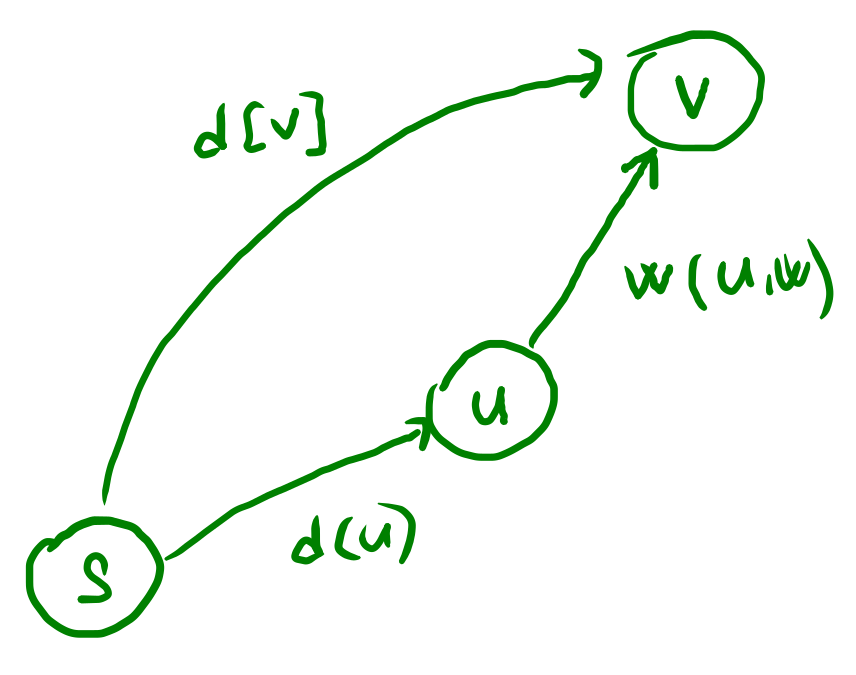
\includegraphics[width=0.4\linewidth]{relax.png}
    \caption{Ukázka činnosti funkce \textit{relax}.}
\end{figure}

%%%%%%%%%%%%%%%%%%%%%%%%%%%%%%%%%%%%%%%%%%%%%%%%%%%%%%%%%%%%%%%%%%%%%%%%%%%%%%%%

\section{Bellman-Fordův algoritmus}

Slouží pro řešení v~obecných grafech, mohou obsahovat cykly a záporné hrany. Záporné cykly je však nutné detekovat a vrátit specifickou hodnotu. V~podstatě se jedná o~\textit{brute force} algoritmus, provede se relaxace $n-1$-krát pro každou hranu.

\bigskip\noindent\begin{minipage}{\linewidth}
\begin{lstlisting}[language=Python, caption={Algoritmus Bellman-Ford. Proč $n-1$ iterací? Protože mezi libovolnými dvěma uzly v~grafu, existuje cesta o~maximálním počtu hran $n-1$.}]
def bellman_ford(G, s, w):
    # G je graf
    # s~je vychozi uzel
    # w je vahova funkce

    # faze inicializace
    initialize_single_source(G, s)
    n = len(G.V) # pocet uzlu

    # faze relaxace: provedeni (n-1) * m relaxaci (m je pocet hran)
    for _ in range(0, n-1):
        for u, v~in G.E:
            relax(u, v, w)

    # faze detekce zaporneho cyklu
    for u, v~in G.E:
        if d[u] > d[v] + w(u, v):
            return NULL

    return pi
\end{lstlisting}
\end{minipage}

\subsection{Složitost}

\begin{compactitem}
    \item Řádek 7, 8 -- $\Theta(1)$.
    \item Řádky 11, 12, 13 -- $(n-1) \cdot \Theta(m) = \Theta(n \cdot m)$, kde $n$ je počet uzlů a $m$ je počet hran grafu.
    \item Řádek 16, 17, 18 -- $\Theta(m)$.
    \item Celkem $\Theta(n \cdot m)$.
\end{compactitem}

\subsection{Příklad}

\begin{figure}[H]
    \centering
    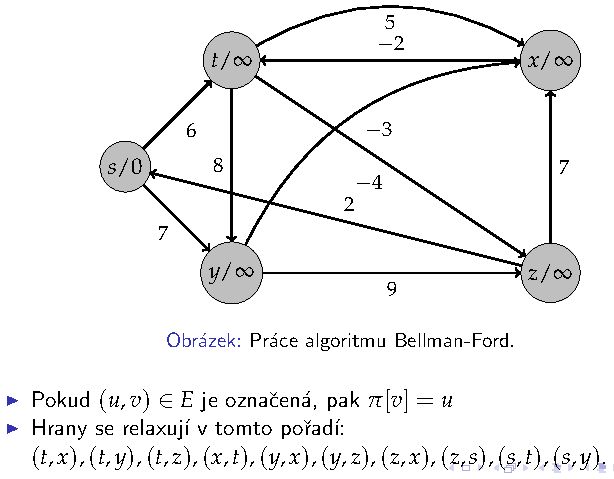
\includegraphics[width=0.75\linewidth]{example_bellman_ford_p1.pdf}
    \caption{Příklad, část 1.}
\end{figure}

\begin{figure}[H]
    \centering
    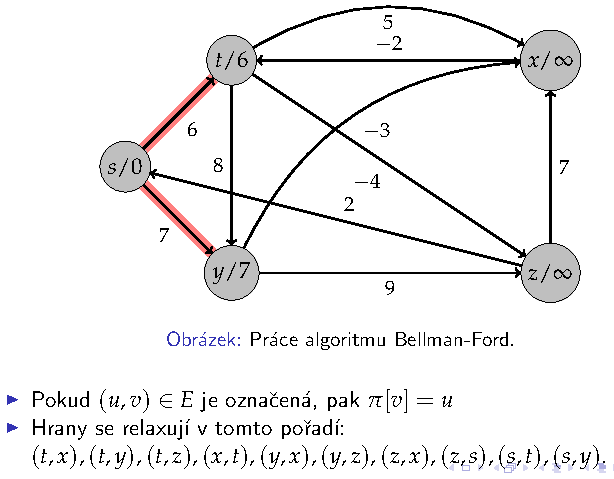
\includegraphics[width=0.75\linewidth]{example_bellman_ford_p2.pdf}
    \caption{Příklad, část 2.}
\end{figure}

\begin{figure}[H]
    \centering
    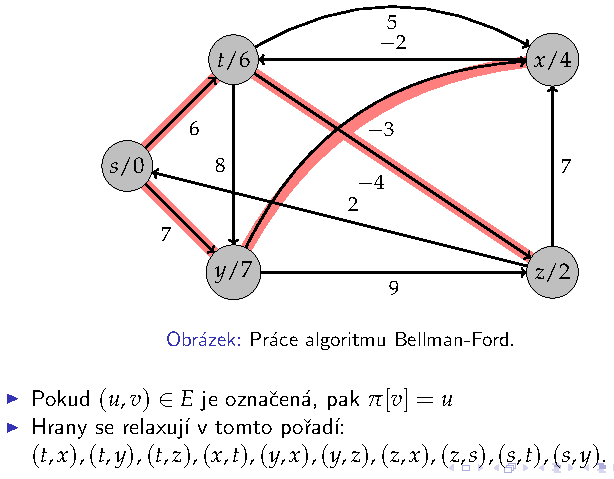
\includegraphics[width=0.75\linewidth]{example_bellman_ford_p3.pdf}
    \caption{Příklad, část 3.}
\end{figure}

\begin{figure}[H]
    \centering
    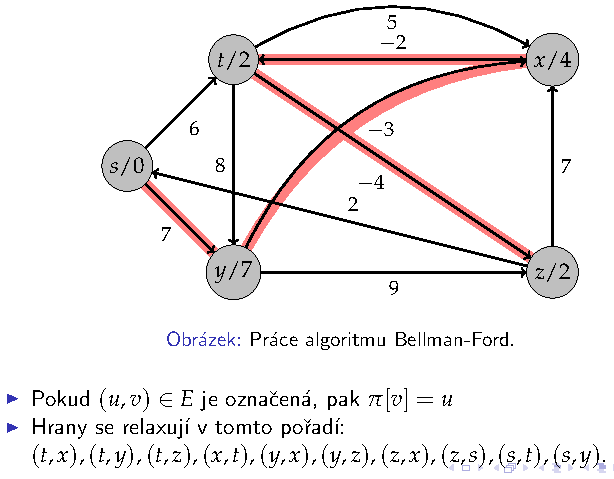
\includegraphics[width=0.75\linewidth]{example_bellman_ford_p4.pdf}
    \caption{Příklad, část 4.}
\end{figure}

\begin{figure}[H]
    \centering
    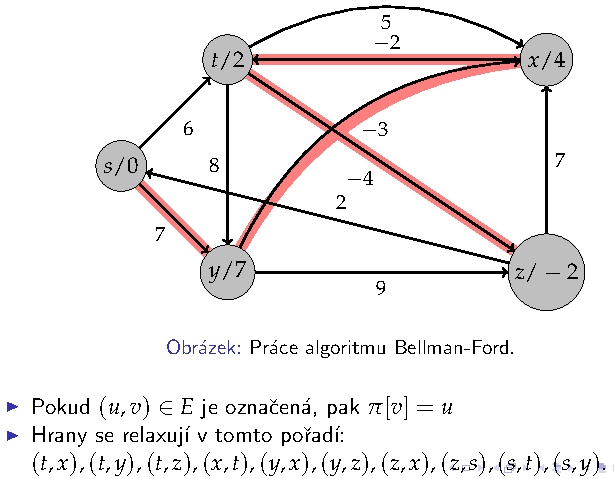
\includegraphics[width=0.75\linewidth]{example_bellman_ford_p5.pdf}
    \caption{Příklad, část 5.}
\end{figure}

%%%%%%%%%%%%%%%%%%%%%%%%%%%%%%%%%%%%%%%%%%%%%%%%%%%%%%%%%%%%%%%%%%%%%%%%%%%%%%%%

\section{Dijkstrův algoritmus}

Slouží pro řešení v~acyklických grafech bez záporných hran. Pro takto omezený problém existují rychlejší algoritmy než pro problém v~obecných grafech.

\bigskip\noindent\begin{minipage}{\linewidth}
\begin{lstlisting}[language=Python, caption={Algoritmus Dijkstra.}]
def dijkstra(G, s, w):
    # G je graf
    # s~je vychozi uzel
    # w je vahova funkce

    # faze inicializace
    initialize_single_source(G, s)
    Q = Queue(G.V) # prioritni fronta uzlu
    S~= {} # mnozina uzlu, ktera uz byla prozkoumana

    # faze relaxace
    while not Q.empty():
        u~= Q.extract_min(d) # vrati prvek z~Q s~nejmensi hodnotou v~d
        S~+= {u}
        # pro vsechny sousedy uzlu u~(Adj je seznam sousedu)
        for v~in Adj[u]:
            relax(u, v, w)

        Q.decrease_key(d) # aktualizace prioritni fronty

    return d, pi
\end{lstlisting}
\end{minipage}

\subsection{Složitost}

\begin{compactitem}
    \item Předpokládejme implementaci prioritní fronty pomocí pole.
    \item Řádek 8, 18 -- $O(1)$.
    \item Řádek 11 -- While cyklus se provede $n$-krát, kde $n$ je počet uzlů.
    \item Řádek 12 -- $O(n)$, najítí minima v~poli uzlů. Celkově (s~cyklem) $O(n^2)$.
    \item Řádek 16 -- $O(m)$, pro všechny hrany. Celkově (s~cyklem) $O(m \cdot n)$.
    \item Celkem $O(n^2 + m) = O(n^2)$.
    \item Pro řídké grafy lze využít implementaci fronty pomocí binární haldy a získat tak $O(m \cdot \log(n))$.
    \item Při implementaci fronty pomocí Fibonacciho haldy dostaneme časovou složitost $O(n \cdot \log(n) + m)$.
\end{compactitem}

\subsection{Příklad}

\begin{figure}[H]
    \centering
    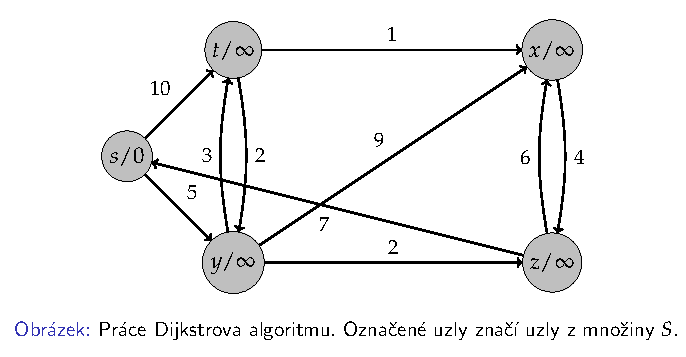
\includegraphics[width=0.80\linewidth]{example_dijkstra_p1.pdf}
    \caption{Příklad, část 1.}
\end{figure}

\begin{figure}[H]
    \centering
    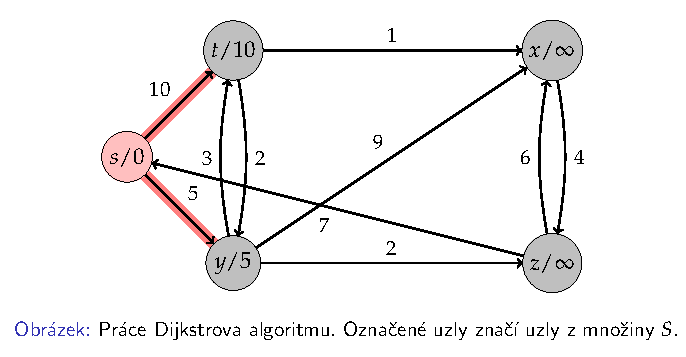
\includegraphics[width=0.80\linewidth]{example_dijkstra_p2.pdf}
    \caption{Příklad, část 2.}
\end{figure}

\begin{figure}[H]
    \centering
    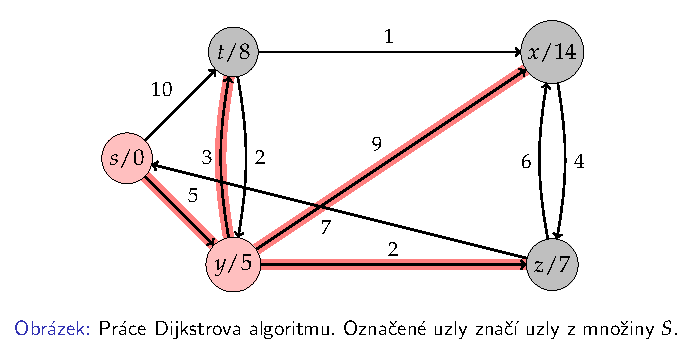
\includegraphics[width=0.80\linewidth]{example_dijkstra_p3.pdf}
    \caption{Příklad, část 3.}
\end{figure}

\begin{figure}[H]
    \centering
    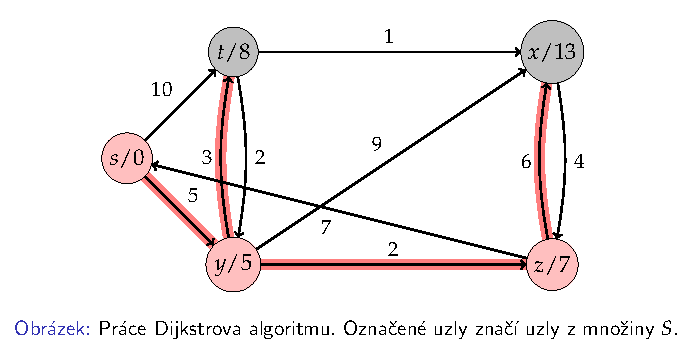
\includegraphics[width=0.80\linewidth]{example_dijkstra_p4.pdf}
    \caption{Příklad, část 4.}
\end{figure}

\begin{figure}[H]
    \centering
    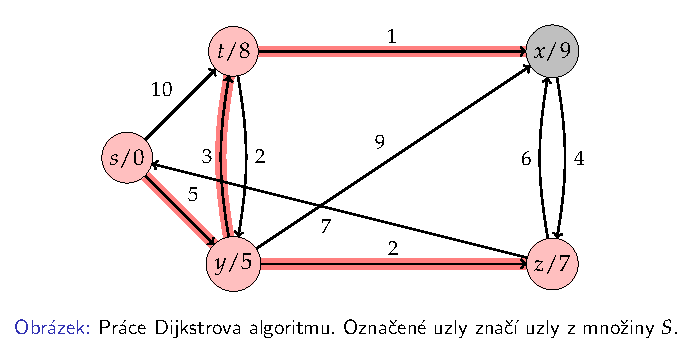
\includegraphics[width=0.80\linewidth]{example_dijkstra_p5.pdf}
    \caption{Příklad, část 5.}
\end{figure}

\begin{figure}[H]
    \centering
    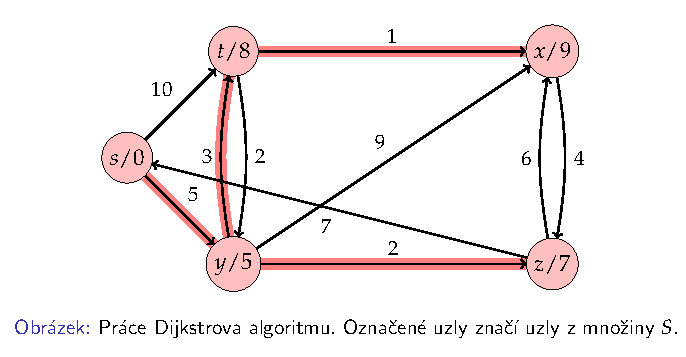
\includegraphics[width=0.80\linewidth]{example_dijkstra_p6.pdf}
    \caption{Příklad, část 6.}
\end{figure}
